\documentclass[oneside,14pt]{extarticle}
\usepackage{cmap}
\usepackage[utf8]{inputenc}
\usepackage{longtable}
\usepackage[english,ukrainian]{babel}
\usepackage{graphicx}
\usepackage{geometry}
\usepackage{listings}
\usepackage{float}
\usepackage{amsmath}
\usepackage{subfig}
\usepackage{tempora}
\renewcommand{\arraystretch}{1.5}
\usepackage{titlesec}
\titleformat{\section}
{\centering\Large\bfseries}{\thesection}{1em}{} % Centered, large, bold font
\geometry{
	a4paper,
	left=20mm,
	right=20mm,
	top=15mm,
	bottom=15mm,
}
\lstset{
	language=c,
	tabsize=4,
	keepspaces,
	showstringspaces=false,
	frame=single,
	breaklines,
	language=C,
}
\graphicspath{ {./pictures} }
\setlength{\parindent}{4em}

\newcommand\subject{Якість програмного забезпечення та тестування}
\newcommand\lecturer{доцент кафедри ПЗ\\Фоменко А.В.}
\newcommand\teacher{асистент кафедри ПЗ\\Джумеля Е.А.}
\newcommand\mygroup{ПЗ-42}
\newcommand\lab{9}
\newcommand\theme{Підсумковий звіт про тестування}
\newcommand\purpose{Розробити підсумковий звіт про тестування}

\begin{document}
\begin{normalsize}
	\begin{titlepage}
		\thispagestyle{empty}
		\begin{center}
			\textbf{МІНІСТЕРСТВО ОСВІТИ І НАУКИ УКРАЇНИ\\
				НАЦІОНАЛЬНИЙ УНІВЕРСИТЕТ "ЛЬВІВСЬКА ПОЛІТЕХНІКА"}
		\end{center}
		\begin{flushright}
			\textbf{ІКНІ}\\
			Кафедра \textbf{ПЗ}
		\end{flushright}
		\vspace{80pt}
		\begin{center}
			\textbf{ЗВІТ}\\
			\vspace{10pt}
			до лабораторної роботи № \lab\\
			\textbf{на тему}: <<\textit{\theme}>>\\
			\textbf{з дисципліни}: <<\subject>>
		\end{center}
		\vspace{80pt}
		\begin{flushright}
			
			\textbf{Лектор}:\\
			\lecturer\\
			\vspace{28pt}
			\textbf{Виконали}:\\
			
			студенти групи \mygroup\\
			Коваленко Д.М.\\
			Снісар В.І.\\
			Баран В.Б.\\
			\vspace{28pt}
			\textbf{Прийняла}:\\
			
			\teacher\\
			
			\vspace{28pt}
			«\rule{1cm}{0.15mm}» \rule{1.5cm}{0.15mm} 2024 р.\\
			$\sum$ = \rule{1cm}{0.15mm}……………\\
			
		\end{flushright}
		\vspace{\fill}
		\begin{center}
			\textbf{Львів – 2024}
		\end{center}
	\end{titlepage}
		
	\begin{description}
		\item[Тема.] \theme.
		\item[Мета.] \purpose.
	\end{description}

    \section*{Лабораторне завдання}
    \begin{enumerate}
    	\item Розробити Summary Test Report модулю, що розробляється, з використанням одного з шаблонів.
    \end{enumerate}
	\section*{Хід роботи}
	\tableofcontents
	\clearpage
	\section{Призначення документа}
	Цей документ описує виконані дії, очікувані та отримані	результати для тестування тестових модулів системи "Віртуальна лабораторія програмної інженерії", а також опис тестової діяльності. Усі ці компоненти є частиною остаточного звіту.
	
	\section{Огляд системи}
	Модуль проектування "Віртуальної лабораторії програмної інженерії" забезпечує студентам та викладачам інструменти для створення, редагування та візуалізації різноманітних діаграм, які використовуються в процесі розробки програмного забезпечення. Основним завданням є підтримка навчання шляхом надання можливостей для практичного застосування теоретичних знань з проектування ПЗ.
	
	Модуль проектування складається з декількох підмодулів, які дозволяють працювати з різними типами UML-діаграм: діаграмами варіантів використання, класів та послідовності.
	
	\begin{itemize}
		\item Редактор діаграм варіантів використання дозволяє додавати акторів, варіанти використання, а також зв'язки між ними.
		\item Редактор діаграм класів підтримує додавання класів, атрибутів, методів та зв’язків між класами.
		\item Редактор діаграм послідовності надає можливість створювати об'єкти, актори, повідомлення та активації.
	\end{itemize}
	
	Функціональні можливості модуля включають збереження діаграм у форматі JSON для подальшого редагування, а також їх експорт для інтеграції з іншими інструментами системи.
	
	\section{Обсяг виконаного тестування}
	У модулі проектування "Віртуальної лабораторії програмної інженерії" будуть наступні підмодулі, які запроектовані, реалізовані та протестовані:
	\begin{itemize}
		\item Редактор діаграм варіантів використання
		\item Редактор діаграм класів
		\item Редактор діаграм послідовності
	\end{itemize}
	
	Тестування інших модулів не передбачено у рамках MVP.
	
	\section{Метрики}
	Для кращої візуалізації виконаної роботи(тестування) представлені
	метрики і вигляді різних графіків. 
	
	\begin{itemize}
		\item Перший графік показує відношення GUI тестів до  Functional  тестів;
		\item Другий графік показує розподіл дефектів за ступенем критичності;
		\item Третій графік показує розподіл дефектів за модулями.
	\end{itemize}
	
	\begin{figure}[H]
		\centering
		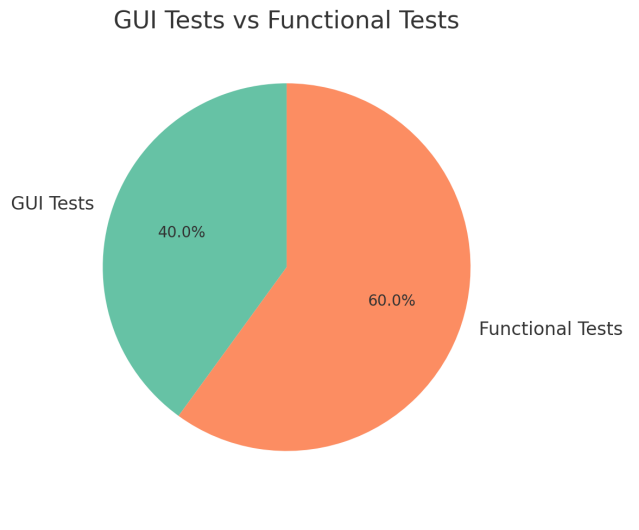
\includegraphics[width=0.7\columnwidth]{1}
		\caption{Відношення GUI тестів до  Functional  тестів}
	\end{figure}
	
	\begin{figure}[H]
		\centering
		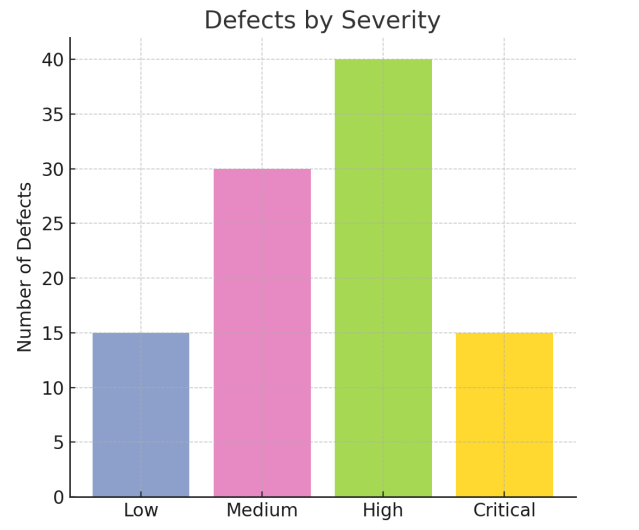
\includegraphics[width=0.7\columnwidth]{2}
		\caption{Розподіл дефектів за ступенем критичності}
	\end{figure}
	
	\begin{figure}[H]
		\centering
		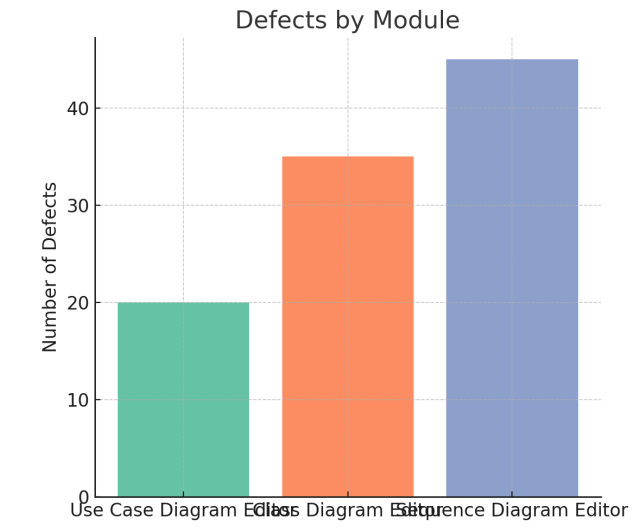
\includegraphics[width=0.7\columnwidth]{3}
		\caption{Розподіл дефектів за модулями}
	\end{figure}
	
	\section{Типи проведених тестів}
	Командою тестувальників було здійснено наступні типи перевірок для модуля проектування "Віртуальної лабораторії програмної інженерії":
	
	\begin{itemize}
		\item Функціональне тестування. Перевірка виконання всього необхідного функціоналу, щоб підтвердити відповідність очікуванням замовника.
		\item Smoke-тестування (димне тестування). Виконане для виявлення явних помилок на початкових етапах роботи модуля.
		\item Модульне тестування (Unit Testing). Тестування кожної атомарної функції в ізольованому середовищі. Використовувались навички автоматизації тестування для створення штучного середовища.
		\item Інтеграційне тестування. Перевірка взаємодії між модулями та їх відповідність вимогам. Використано перевірені модулі, згруповані у множини.
		\item Тестування інтерфейсу (GUI). Оцінка інтуїтивності інтерфейсу, адаптивності для людей різного віку та користувачів з обмеженнями, наприклад, з дальтонізмом.
		\item Performance тестування. Тестування продуктивності та стресостійкості модуля під великим навантаженням.
	\end{itemize}
	
	Результати тестування: Модуль проектування відповідає вимогам та готовий до використання в навчальному процесі.
	
	\section{Тестове середовище та інструменти}
	Для написання тестів було використано середовище розробки IntelliJ. Фреймворк JUnit 5 застосовувався для виконання тестів. Серверна частина системи працювала на Tomcat, а база даних — на H2 in-memory database.
	
	Тестування серверної частини проводилося на ОС Mac Ventura 13.0 (22A380). Клієнтська частина тестувалася на ОС Windows 10 у браузері Google Chrome (версія 109.0.5391.0, 64-bit).
	
	\section{Вивчені уроки}
	\begin{enumerate}
		\item Проактивне тестування. Щоб уникнути дороговартісних виправлень у майбутньому, тестування слід розпочинати одразу після початку розробки.
		\item Тісна співпраця з розробниками. Співпраця з розробниками допомагає краще розуміти код та алгоритми, особливо при недостачі документації. Це забезпечує якісне написання автоматизованих тестів і виконання тест-кейсів "білої скриньки".
		\item Дотримання процесу. Важливо дотримуватися процесу передачі коду на тестування та аналізувати результати відповідальними особами для якісної розробки ПЗ.
		\item Готовність до тестування:
		\begin{itemize}
			\item доступний повний або частковий код для тестування;
			\item вимоги визначені та затверджені;
			\item наявні потрібні тестові дані;
			\item тест-кейси розроблені та готові;
			\item тестове середовище налаштоване, а також доступні всі необхідні ресурси та інструменти.
		\end{itemize}
	\end{enumerate}
	
	\section{Рекомендації}
	Тестувальна документація має бути чіткою і відслідковуватися Lead QA у Confluence. Процес тестування слід розпочинати з початком імплементації. Необхідна ефективна комунікація з боку менеджменту. Test Case'и повинні створюватися в QTest на основі Acceptance Criteria, зазначених у Jira для кожної story, bug або task. Недоліки слід якісно документувати і передавати на виправлення одразу після їх виявлення.
	
	\section{Найкращі методи}
	Тестові сценарії спроектовані для забезпечення повного покриття всіх аспектів ПЗ у певному або випадковому порядку. Важливим є збір і аналіз точних даних, починаючи з розробки детальних користувацьких інструкцій і списку завдань.
	
	\section{Критерії релізу системи}
	\begin{itemize}
		\item Дотримано терміни або вичерпано бюджет.
		\item Виконано та задокументовано всі тест-кейси.
		\item Вимоги повністю покриті під час тестування.
		\item Усі дефекти виправлено і перетестовано.
		\item Відсутні критичні помилки з високим пріоритетом або серйозністю.
	\end{itemize}
	
	\section{Підпис}
	За результатами тестування, на основі відгуків користувачів та замовника, команда ухвалила рішення про публікацію робочої версії застосунку.
	
	\section{Визначення, абревіатури та скорочення}
	\begin{itemize}
		\item Jira — система для відстеження помилок, організації спілкування та управління проєктами.
		\item ОС — операційна система.
		\item GUI — графічний інтерфейс користувача.
		\item MVP — мінімально життєздатний продукт.
	\end{itemize}
	
	\section*{Висновки}
	Під час виконання лабораторної роботи створено підсумковий звіт про процес та результати тестування розробленого модуля проектування для "Віртуальної лабораторії". У даному документі є інформація про результати тестування, метрики покриття якості, кількості дефектів та їх відношення, тестове середовище і використані інструменти. 
	    
	
\end{normalsize}
\end{document}
